\documentclass{article}
\usepackage[utf8]{inputenc}
\usepackage{array,multirow,graphicx}
\usepackage{amsmath,amssymb,latexsym}
\usepackage{mathabx}
\usepackage{parskip}
\usepackage{listings}
\usepackage[section]{placeins}
\usepackage{hyperref}
\usepackage[english]{babel}
\usepackage{biblatex}
\renewcommand{\sfdefault}{ptm}
\graphicspath{ {/} }

\title{Report.11.DB.Design.NGO}
\author{Linh Duong}
\date{November 2017}

\begin{document}

\maketitle

\section{Database design}
\subsection{Determine concepts}
\begin{itemize}
    \item Head office
    \item Project
    \item Action 
    \item City
\end{itemize}

\subsection{Determine attributes}
\begin{itemize}
    \item Head office 
    \subitem office\_id
    % \subitem city
    \subitem address
    \subitem phone\_number
    \subitem director
    
    \item Project
    \subitem code
    \subitem title 
    \subitem date of beginning
    \subitem date of ending 
    \subitem budget
    \subitem person\_in\_charge 
    
    \item Action 
    % \subitem name
    % \subitem city
    \subitem investment
    \subitem description 
    
    \item City
    \subitem city\_id
    \subitem name
    \subitem country 
    \subitem inhabitant 
\end{itemize}

\subsection{Determine links}
\begin{itemize}
    \item City and Head office (locates)
    \item Project and Head office (manages)
    \item Action and Project (has)
    \item City and Action (realized)
\end{itemize}

\subsection{Determine types}
\begin{itemize}
    \item Head office 
    \subitem office\_id INT 
    % \subitem city
    \subitem address VARCHAR(50)
    \subitem phone\_number VARCHAR(20)
    \subitem director VARCHAR(50)
    
    \item Project
    \subitem code INT 
    \subitem title VARCHAR(200)
    \subitem date of beginning (DATE)
    \subitem date of ending  (DATE)
    \subitem budget (INT)
    \subitem person\_in\_charge VARCHAR(50)
    
    \item Action 
    % \subitem name VARCHAR(50)
    % \subitem city
    \subitem investment INT 
    \subitem description VARCHAR(200)
    
    \item City
    \subitem city\_id INT 
    \subitem name VARCHAR(20)
    \subitem country VARCHAR(20)
    \subitem inhabitant INT
\end{itemize}

\subsection{Solve foreign key links}
\begin{itemize}
    \item Head office 
    \subitem office\_id INT 
    \subitem city\_id INT
    \subitem address VARCHAR(50)
    \subitem phone\_number VARCHAR(20)
    \subitem director VARCHAR(50)
    
    \item Project
    \subitem code INT 
    \subitem office\_id INT
    \subitem title VARCHAR(200)
    \subitem date of beginning (DATE)
    \subitem date of ending  (DATE)
    \subitem budget (INT)
    \subitem person\_in\_charge VARCHAR(50)
    
    \item Action 
    \subitem act\_id INT
    \subitem code INT
    \subitem description VARCHAR(200)
    
    \item City
    \subitem city\_id INT 
    \subitem name VARCHAR(20)
    \subitem country VARCHAR(20)
    \subitem inhabitant INT
    
    \item ActionCity 
    \subitem act\_id
    \subitem city\_id
    \subitem investment INT 
    
    
\end{itemize}
\section{Implementation}
\begin{lstlisting}[language=sql]
create database if not exists NGO;

use NGO;

create table city (
city_id int not null auto_increment,
name varchar(20), 
country varchar(20), 
inhabitant int ,
primary key (city_id)
);

create table office (
office_id int not null auto_increment, 
city_id int not null ,
address varchar(50), 
phong_number varchar(20), 
director varchar(50), 
primary key (office_id),
foreign key (city_id) references city(city_id)
);

create table project (
code int not null auto_increment, 
office_id int, 
title varchar(200), 
begin_date date , 
end_date date, 
budget int, 
person_in_charge varchar(50), 
primary key (code), 
foreign key (office_id) references office(office_id)
);

create table action (
act_id int not null auto_increment, 
code int , 
description varchar(200), 
primary key (act_id), 
foreign key (code) references project(code)
);

create table action_city (
act_id int, 
city_id int, 
investment int,
foreign key (act_id) references action(act_id), 
foreign key (city_id) references city(city_id)
);
\end{lstlisting}

\section{Describe tables}
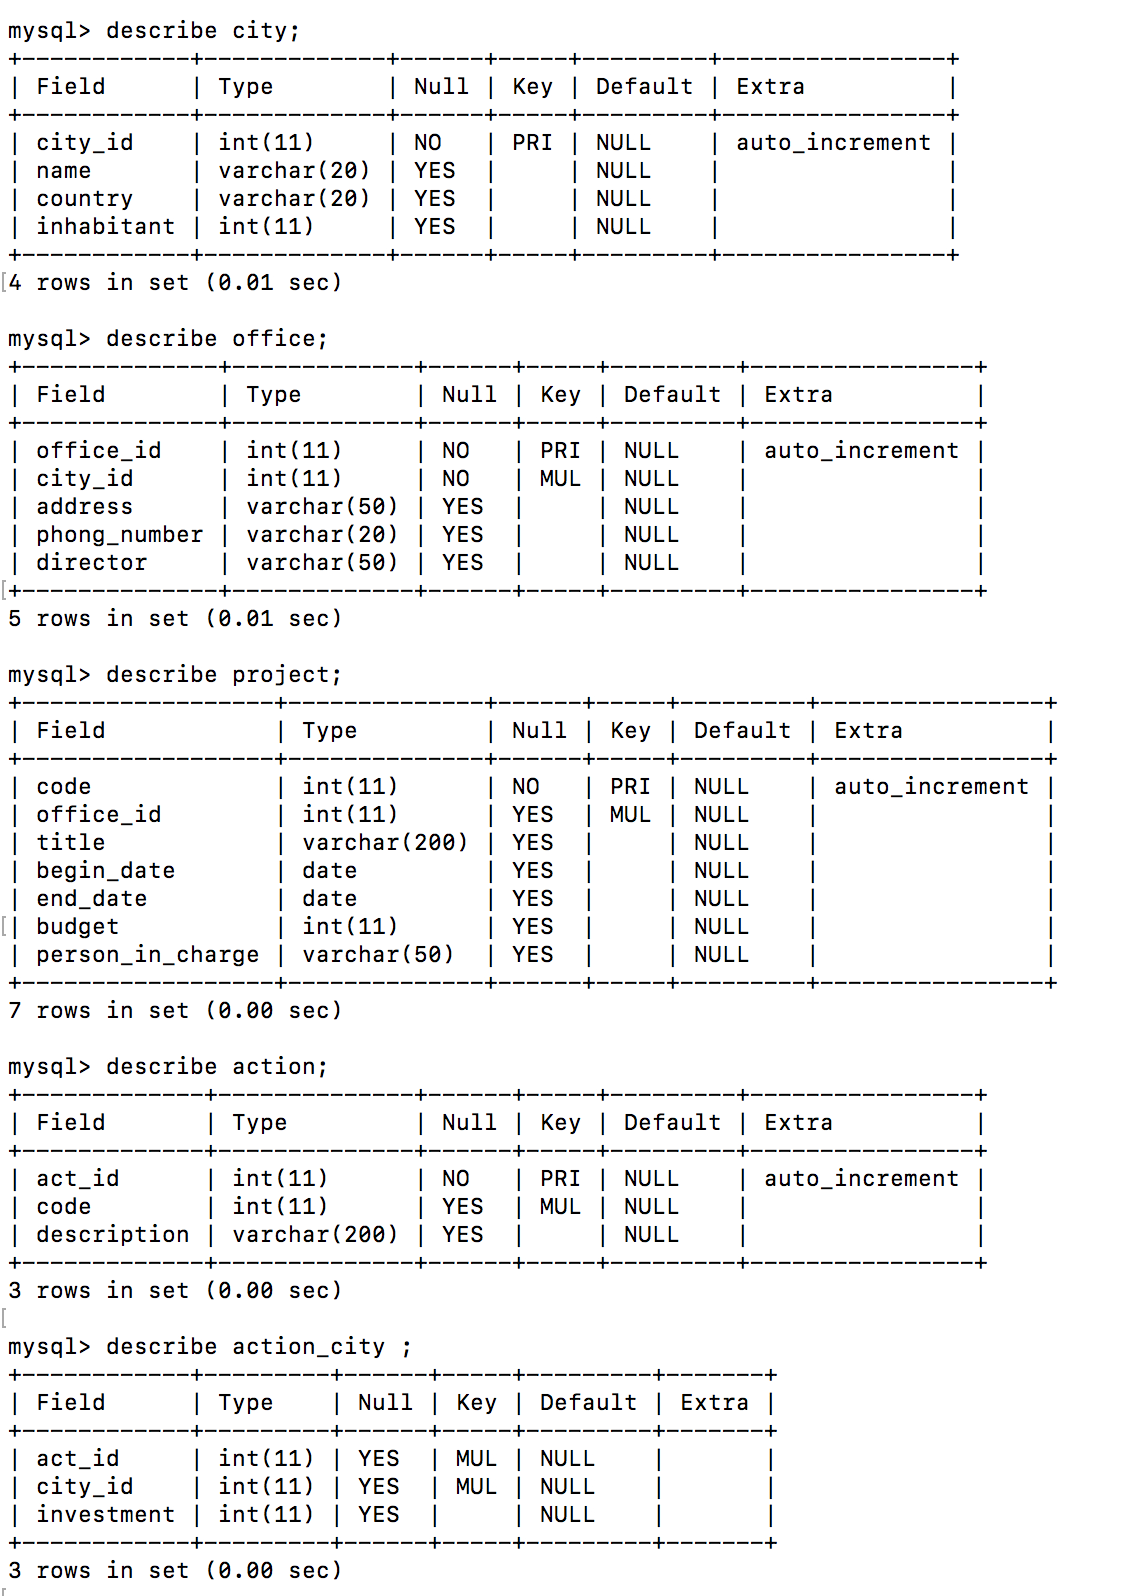
\includegraphics[width=\linewidth]{describe2.png}



\end{document}
